\documentclass{beamer}
%Imports and customization
\usepackage{tikz}
\usepackage{graphicx}
\usepackage{tikz-feynman}
\usepackage{ulem}
\usepackage{colortbl}
\graphicspath{ 
    {./images/}
}

\beamertemplatenavigationsymbolsempty
\setbeamertemplate{sidebar right}{}
\setbeamertemplate{footline}{
    \hfill\usebeamertemplate***{navigation symbols}
    \hspace{1cm}\insertframenumber{}/\inserttotalframenumber
}
\setbeamertemplate{caption}{\raggedright\insertcaption\par}
\setbeamersize{text margin left=4mm,text margin right=4mm} 

\setbeamerfont{itemize/enumerate body}{size=\scriptsize}
\setbeamerfont{itemize/enumerate subbody}{size=\scriptsize}
\setbeamerfont{itemize/enumerate subsubbody}{size=\scriptsize}


%Custom Macros
\newcommand{\statwarn}{
    \tiny \color{red} Absolute numbers here mean NOTHING. Plots are based on small (100k events) samples, and are highly biased. All that matters is relative position!
}


% WARNING: When using these commands, the image argument must
% NOT have spaces between itself and the braces
\newcommand{\fullscreenimage}[2]{
    \frame{
        \frametitle{#1} 
        \begin{figure}
        \includegraphics[height=0.9\textheight,width=\textwidth,keepaspectratio]{#2}
        \end{figure}
    }
}


\newcommand{\importpdf}[3]{
    \frame{
        \begin{columns}\column{\dimexpr\paperwidth-10pt}
        \begin{figure}
        \includegraphics[page=#2,height=0.8\textheight,width=\textwidth,keepaspectratio]{#1}
        \end{figure}

        {\tiny #3}
        \end{columns}
    }
}


\newcommand{\displayone}[3]{
    \frame{
        \frametitle{#1} 
        \begin{columns}
            \begin{column}{0.5\textwidth}
                #2
            \end{column}
            \begin{column}{0.5\textwidth}
                \begin{figure}
                    \includegraphics[width=\linewidth,height=\textheight,keepaspectratio]{#3}
                \end{figure}
            \end{column}
        \end{columns}
    }
}

\newcommand{\displayonelarge}[3]{
    \frame{
        \frametitle{#1} 
        \begin{columns}
            \begin{column}{0.3\textwidth}
                #2
            \end{column}
            \begin{column}{0.7\textwidth}
                \begin{figure}
                    \includegraphics[width=\linewidth,height=0.8\textheight,keepaspectratio]{#3}
                \end{figure}
            \end{column}
        \end{columns}
    }
}


\newcommand{\displaytwo}[4]{
    \frame{
        \frametitle{#1} 
        #2
        \begin{columns}
            \begin{column}{0.5\textwidth}
                \begin{figure}
                    \includegraphics[width=\linewidth,height=\textheight,keepaspectratio]{#3}
                \end{figure}
            \end{column}
            \begin{column}{0.5\textwidth}
                \begin{figure}
                    \includegraphics[width=\linewidth,height=\textheight,keepaspectratio]{#4}
                \end{figure}
            \end{column}
        \end{columns}
    }
}

\newcommand{\displaytwocaption}[6]{
    \frame{
        \frametitle{#1} 
        #2
        \begin{columns}
            \begin{column}{0.5\textwidth}
                \begin{figure}
                    \includegraphics[width=\linewidth,height=\textheight,keepaspectratio]{#3}
                    \caption{#4}
                \end{figure}
            \end{column}
            \begin{column}{0.5\textwidth}
                \begin{figure}
                    \includegraphics[width=\linewidth,height=\textheight,keepaspectratio]{#5}
                    \caption{#6}
                \end{figure}
            \end{column}
        \end{columns}
    }
}

\newcommand{\displaytwoVcaption}[6]{
    \frame{
        \begin{columns}
            \begin{column}{0.5\textwidth}
                \frametitle{#1} 
                #2
            \end{column}
            \begin{column}{0.5\textwidth}
                \begin{figure}
                    \includegraphics[width=\linewidth,height=0.3\textheight,keepaspectratio]{#3}
                    \caption{#4}
                \end{figure}

                \begin{figure}
                    \includegraphics[width=\linewidth,height=0.3\textheight,keepaspectratio]{#5}
                    \caption{#6}
                \end{figure}
            \end{column}
        \end{columns}
    }
}


\newcommand{\displaythree}[5]{
    \frame{
        \begin{columns}[T]
            \begin{column}{0.4\textwidth}
                {\usebeamercolor[fg]{title} \insertframetitle{#1} }\\
                \vspace{5mm}
                #2
            \end{column}
            \begin{column}{0.4\textwidth}
                \begin{figure}
                    \includegraphics[width=\linewidth,height=\textheight,keepaspectratio]{#3}
                \end{figure}
            \end{column}
        \end{columns}
        \begin{columns}[T]
            \begin{column}{0.4\textwidth}
                \begin{figure}
                    \includegraphics[width=\linewidth,height=\textheight,keepaspectratio]{#4}
                \end{figure}
            \end{column}
            \begin{column}{0.4\textwidth}
                \begin{figure}
                    \includegraphics[width=\linewidth,height=\textheight,keepaspectratio]{#5}
                \end{figure}
            \end{column}
        \end{columns}
    }
}


\newcommand{\displayfour}[5]{
    \frame{
        \frametitle{#1} 
        \begin{columns}[T]
            \begin{column}{0.4\textwidth}
                \begin{figure}
                    \includegraphics[width=\linewidth,height=\textheight,keepaspectratio]{#2}
                \end{figure}
            \end{column}
            \begin{column}{0.4\textwidth}
                \begin{figure}
                    \includegraphics[width=\linewidth,height=\textheight,keepaspectratio]{#3}
                \end{figure}
            \end{column}
        \end{columns}
        \begin{columns}[T]
            \begin{column}{0.4\textwidth}
                \begin{figure}
                    \includegraphics[width=\linewidth,height=\textheight,keepaspectratio]{#4}
                \end{figure}
            \end{column}
            \begin{column}{0.4\textwidth}
                \begin{figure}
                    \includegraphics[width=\linewidth,height=\textheight,keepaspectratio]{#5}
                \end{figure}
            \end{column}
        \end{columns}
    }
}


\newcommand{\pstrike}[2]{
    \only<-\the\numexpr#1-1>{#2}
    \only<#1->{\sout{#2}}
}


\newcommand{\announcesection}[1]{
    \section{#1}
    \frame{
        \begin{center}
            {\huge #1} 
        \end{center}
    }
}

\newcommand{\kvv}{\kappa_{2V}}
\newcommand{\kl}{\kappa_{\lambda}}
\newcommand{\kv}{\kappa_{V}}

\newcommand{\fkvv}[1]{\kappa_{2V,#1}}
\newcommand{\fkl} [1]{\kappa_{\lambda,#1}}
\newcommand{\fkv} [1]{\kappa_{V,#1}}

\newcommand{\importpdfwpages}[3]{
    \foreach \pageN in {#2,...,#3}{
        \importpdf{#1}{\pageN}{}
    }
}

\newcommand{\hyper}[2]{{\color{blue}\href{#1}{#2}}}



%Begin Presentation
\begin{document}
\title{Incorporating the FTK into the B-Jet Trigger}   
\author{
    Chris Milke (SMU),\\
    on behalf of the B-Jet Trigger Group
} 
\date{31 July, 2019} 

\frame{\titlepage} 
\frame{\frametitle{Overview} \tableofcontents}

%intro
\section{Background}

\frame{
    \frametitle{ Offline to Online: The B-Jet Trigger Retuning Process }
    \begin{figure}
        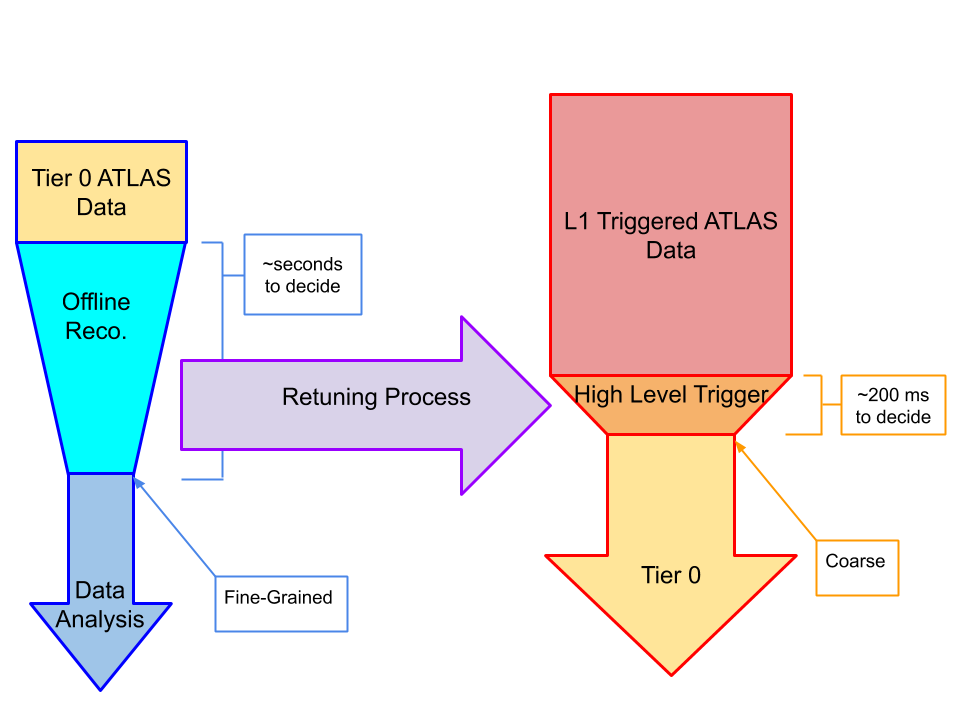
\includegraphics[width=\linewidth,height=\textheight,keepaspectratio]{offline_to_online}
    \end{figure}
}


\frame{
    \frametitle{ Details of the Retuning Process }
    \begin{figure}
        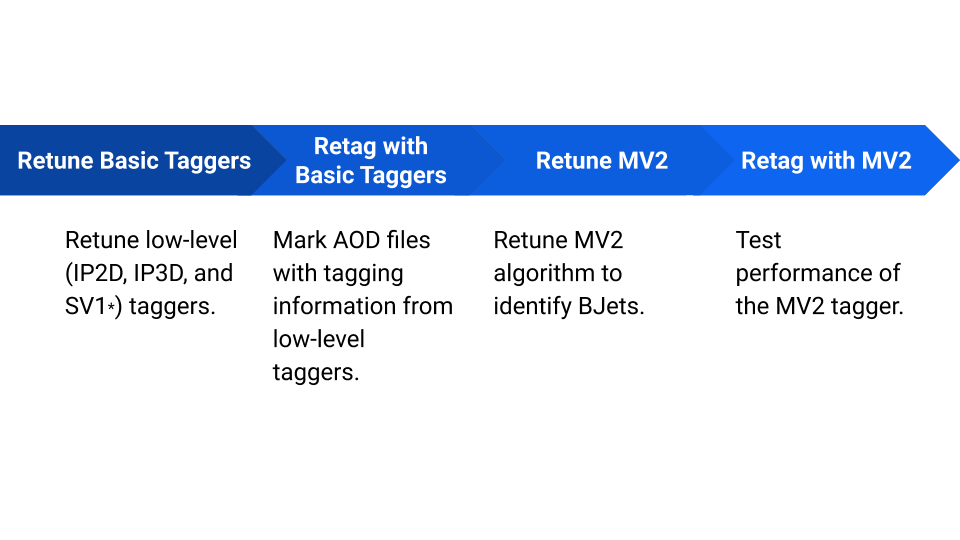
\includegraphics[width=\linewidth,height=\textheight,keepaspectratio]{retune_process}
    \end{figure}
}

\announcesection{Tagger Performance} 
\displayone{ MV2c10 Performance }
    { \begin{itemize}
        \item Black curve is official calibration used in 2018 data taking
        \item Blue curve retuned using 4 Million ttbar monte carlo (production 410470)
        \item Blue and black tuned on different ttbar samples, so consistent performance is reassuring
        \item Primary objective is raise FTK performance closer to HLT levels
        \item FTKRefit-IDTrig shows little difference compared to FTK-IDTrig
    \end{itemize} }
    {btag_c10_score_comparison/mv2c10_roc_ttbar}

\displaytwo{ IP2D and IP3D Performance }
    { \begin{itemize}
        \item MV2c10 is a product of these two (among other variables)
        \item Both Taggers show performance issues for FTK
        \item As FTKRefit-IDTrig is not distinct from FTK-IDTrig,
            it will be omitted from further plots
    \end{itemize} }
    {ipxd_performance/performance_roc_ttbar_ip2d}
    {ipxd_performance/performance_roc_ttbar_ip3d}

\displaythree{Comparison of $d0$}
    { \begin{itemize}
        \item Significance is what is ultimately used in tagging
        \item Significance = d0 / error
        \item d0 Error for FTK-IDTrig appears "shifted"
        \item Unsure if this is a source of performance discrepencies
    \end{itemize} }
    {track_study/plot_d0_0}
    {track_study/plot_d0_err_0}
    {track_study/plot_d0_sig_0}
\displaythree{Comparison of $z0$}{}
    {track_study/plot_z0_0}
    {track_study/plot_z0_err_0}
    {track_study/plot_z0_sig_0}

\frame{
    \frametitle{Performance Summary}
    \begin{itemize} {\normalsize 
        \item MV2c10 FTK-IDTrig performance is significantly lower than HLT performance
        \item Low-level taggers (IPxD) use fewer variables,
            making them a useful probe into underlying issues
        \item IP2D and IP3D taggers depend on track
            Impact Parameter values $d_0$ and $z_0\sin\theta$ respectively
    } \end{itemize}
}
\announcesection{Jet Correlation Study}

\fullscreenimage{rejection_efficiency_lock}
\displaytwo{Selecting the Appropriate LLR Cut}{rejection_level}{rejection_level_zoom}

\announcesection{Results of Jet Correlation Study}
\fullscreenimage{correlation_rubric}

\fullscreenimage{correlation_pt}
\fullscreenimage{correlation_phi}
\fullscreenimage{correlation_theta}
\fullscreenimage{correlation_d0}
\fullscreenimage{correlation_d0_err}
\fullscreenimage{correlation_d0_sig}

\fullscreenimage{correlation_numPixelDeadSensors_0}
\fullscreenimage{correlation_numPixelHits_0}
\fullscreenimage{correlation_numPixelHoles_0}
\fullscreenimage{correlation_numSCTDeadSensors_0}
\fullscreenimage{correlation_numSCTHits_0}
\fullscreenimage{correlation_numSCTHoles_0}
\frame{
    \begin{figure}
    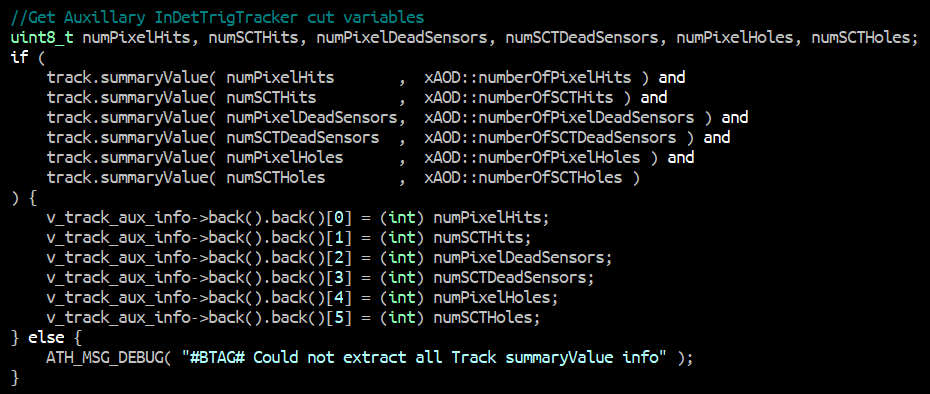
\includegraphics[width=\linewidth,height=\textheight,keepaspectratio]{quality_cut_retrieval}
    \caption{
        \url{https://gitlab.cern.ch/atlas-trigger/b-jet/TrigBtagAnalysis/blob/master/src/BTriggerTuning.cxx\#L1160}
    }
    \end{figure}
}

\frame{
    \frametitle{Track Quality Values}

    Track quality values appear to have no effect on performance at all

    \begin{columns}[T]
        \begin{column}{0.33\textwidth}
            \begin{figure}
                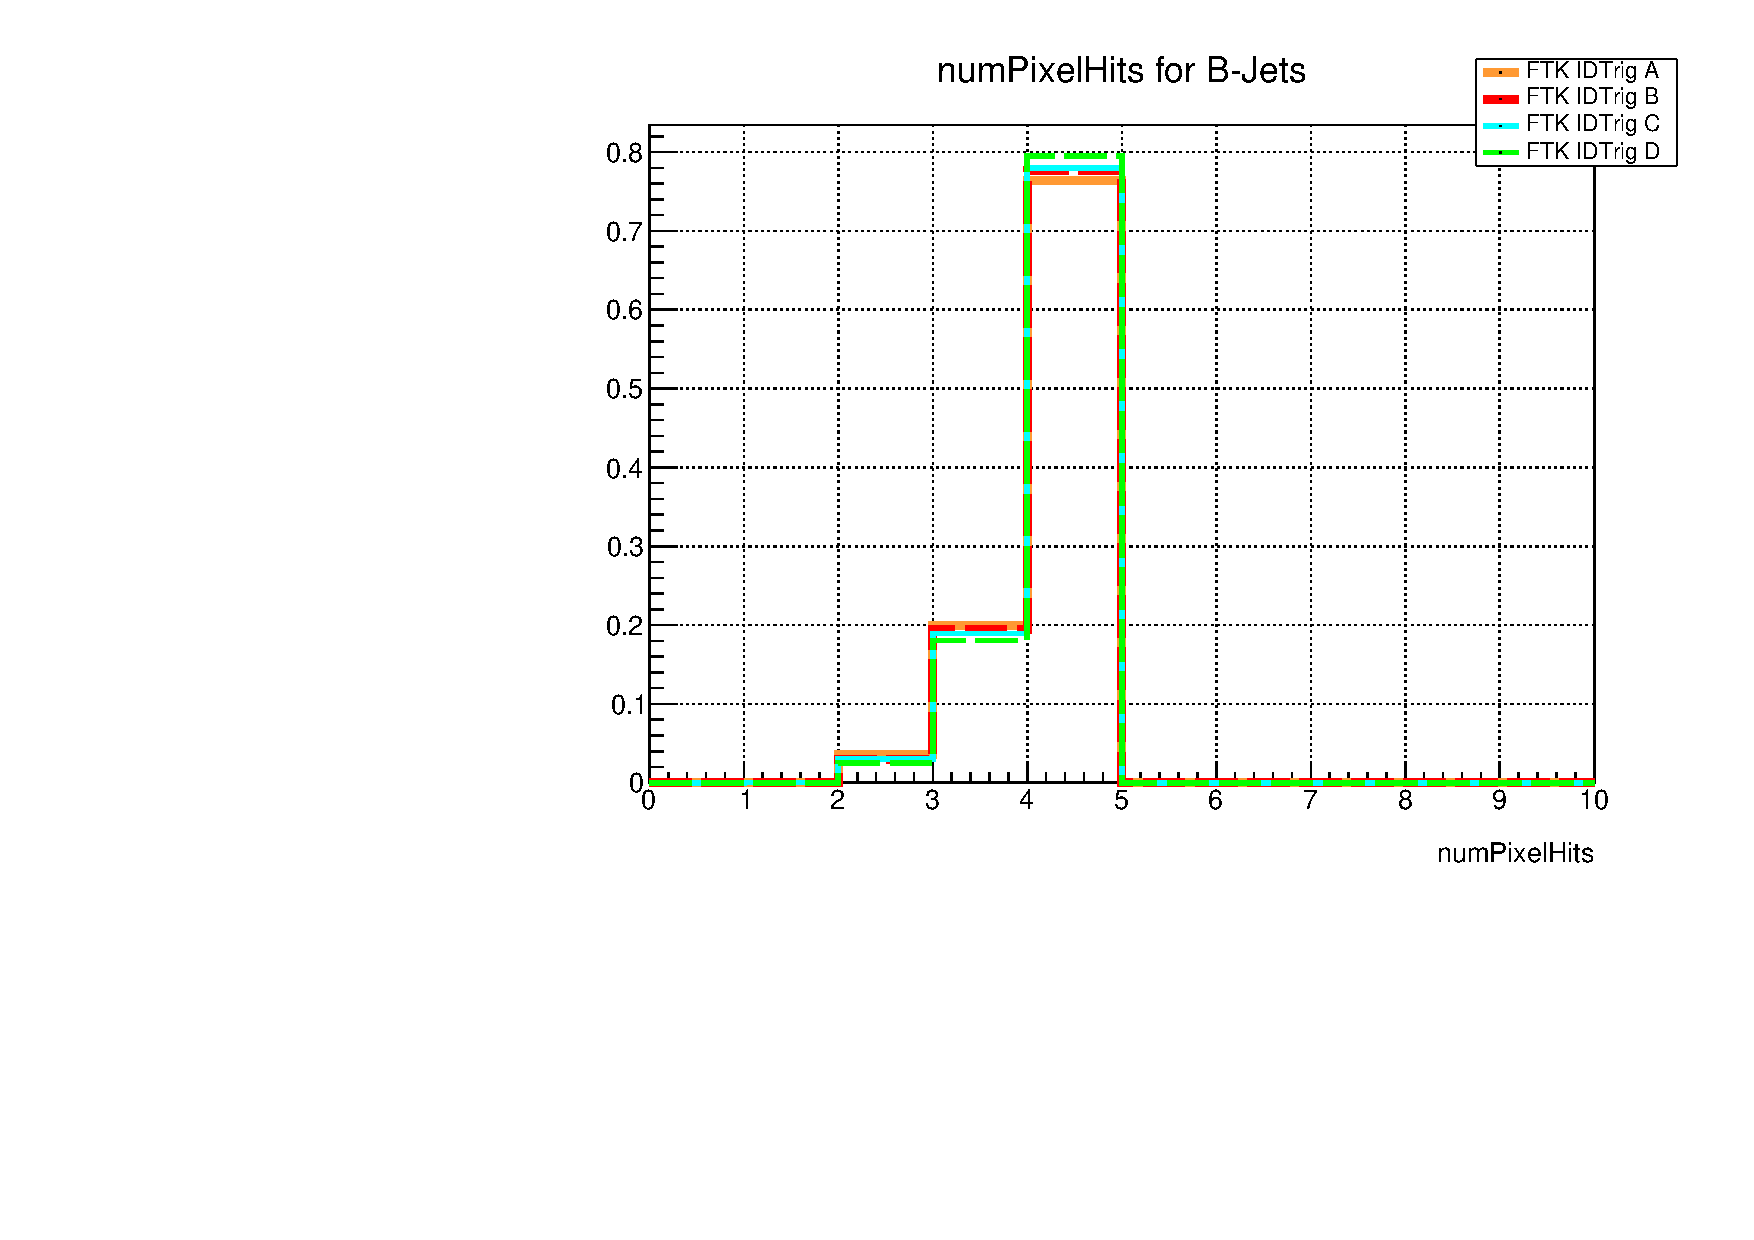
\includegraphics
                [width=\linewidth,height=\textheight,keepaspectratio]
                {correlation_numPixelHits_0}
            \end{figure}
            \begin{figure}
                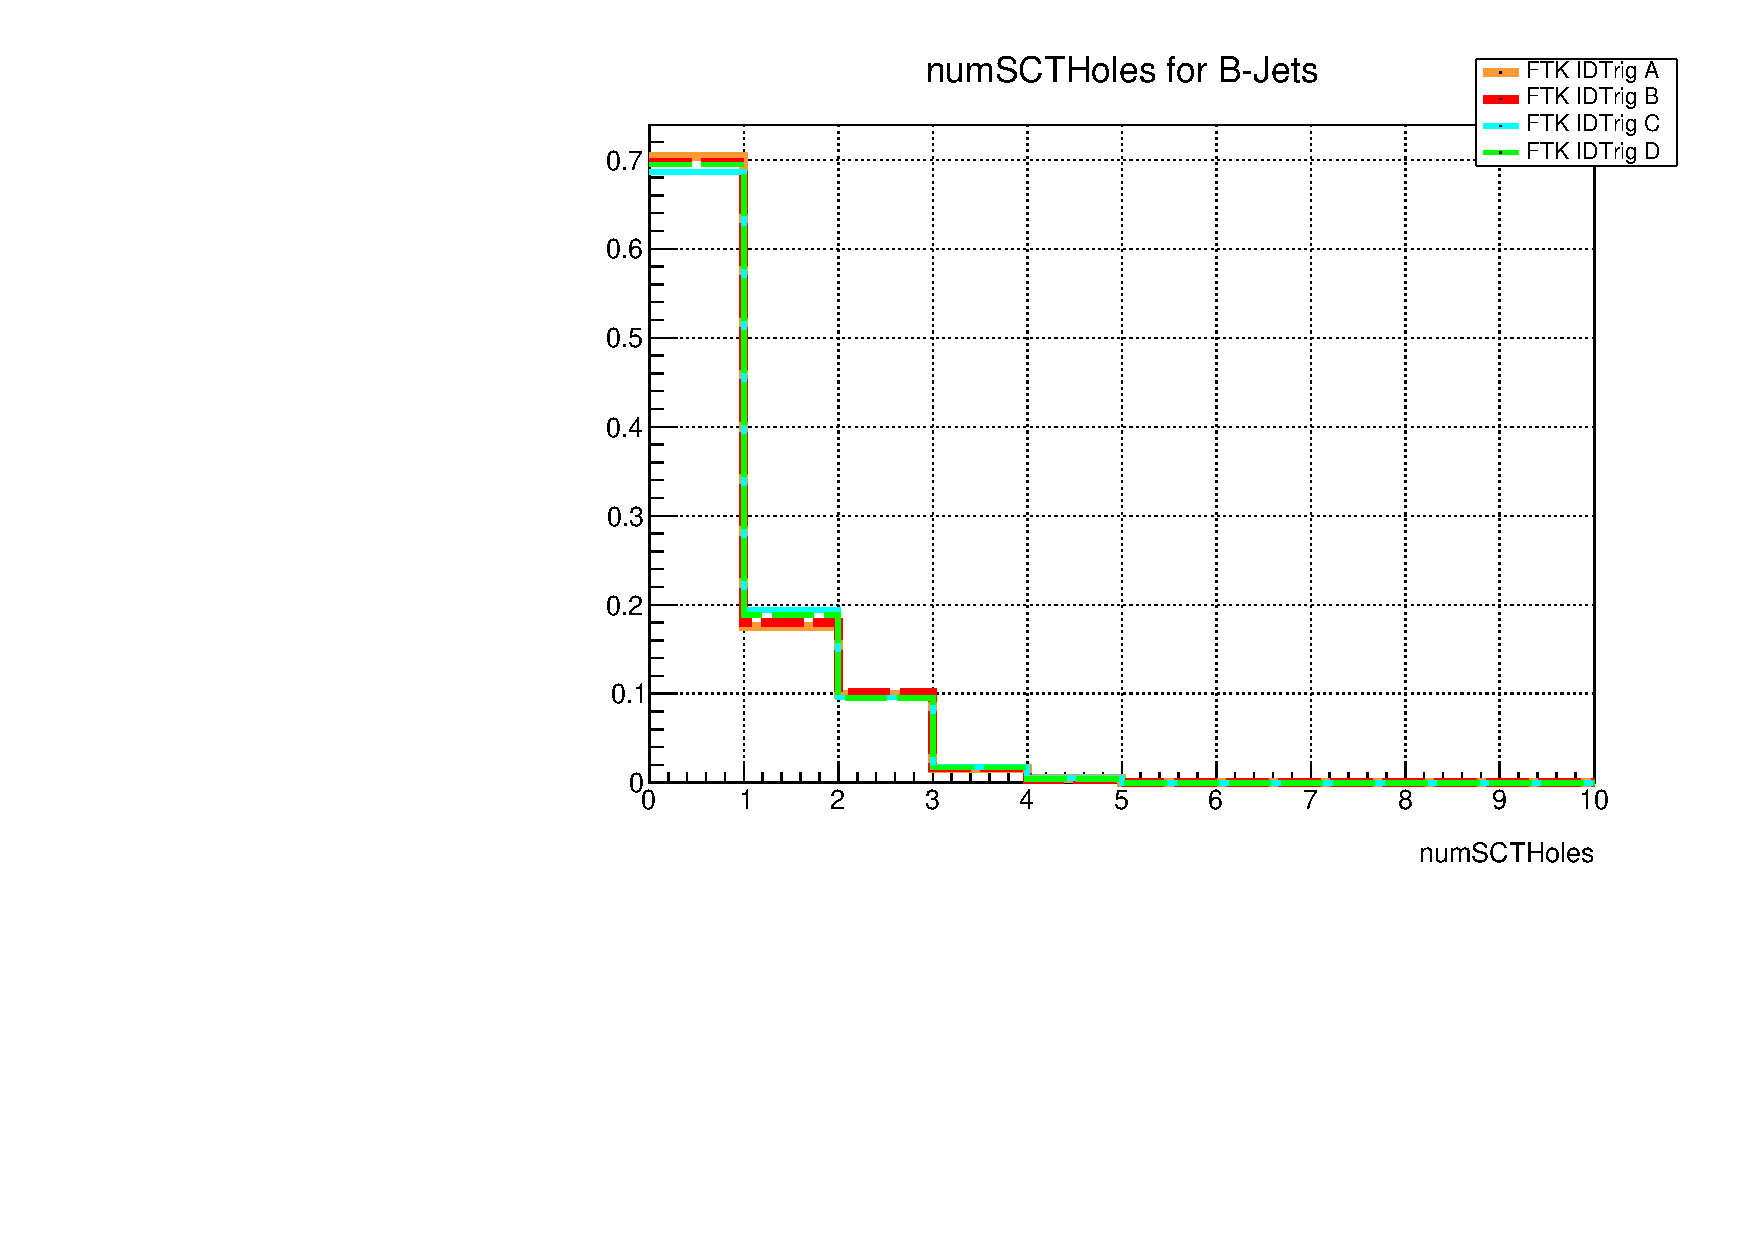
\includegraphics
                [width=\linewidth,height=\textheight,keepaspectratio]
                {correlation_numSCTHoles_0}
            \end{figure}
        \end{column}
        \begin{column}{0.33\textwidth}
            \begin{figure}
                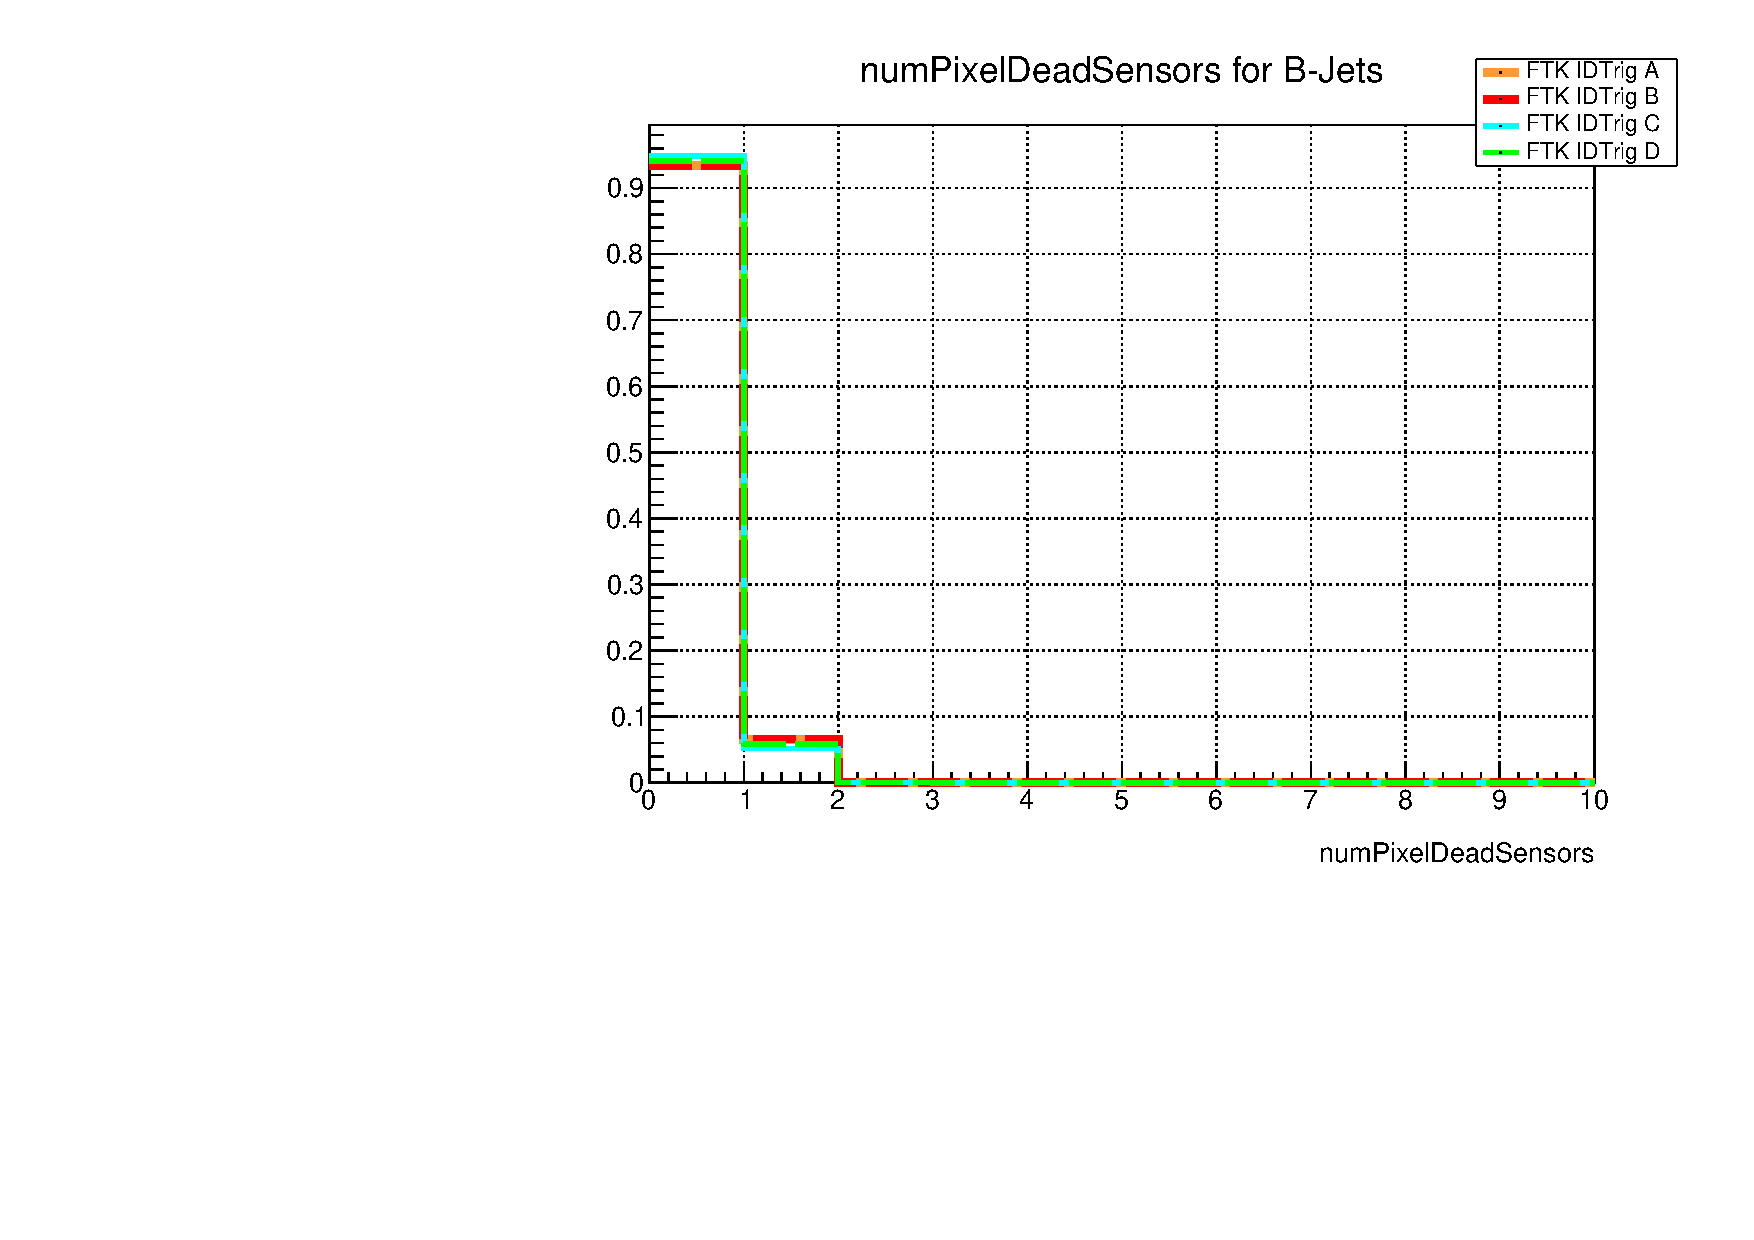
\includegraphics
                [width=\linewidth,height=\textheight,keepaspectratio]
                {correlation_numPixelDeadSensors_0}
            \end{figure}
            \begin{figure}
                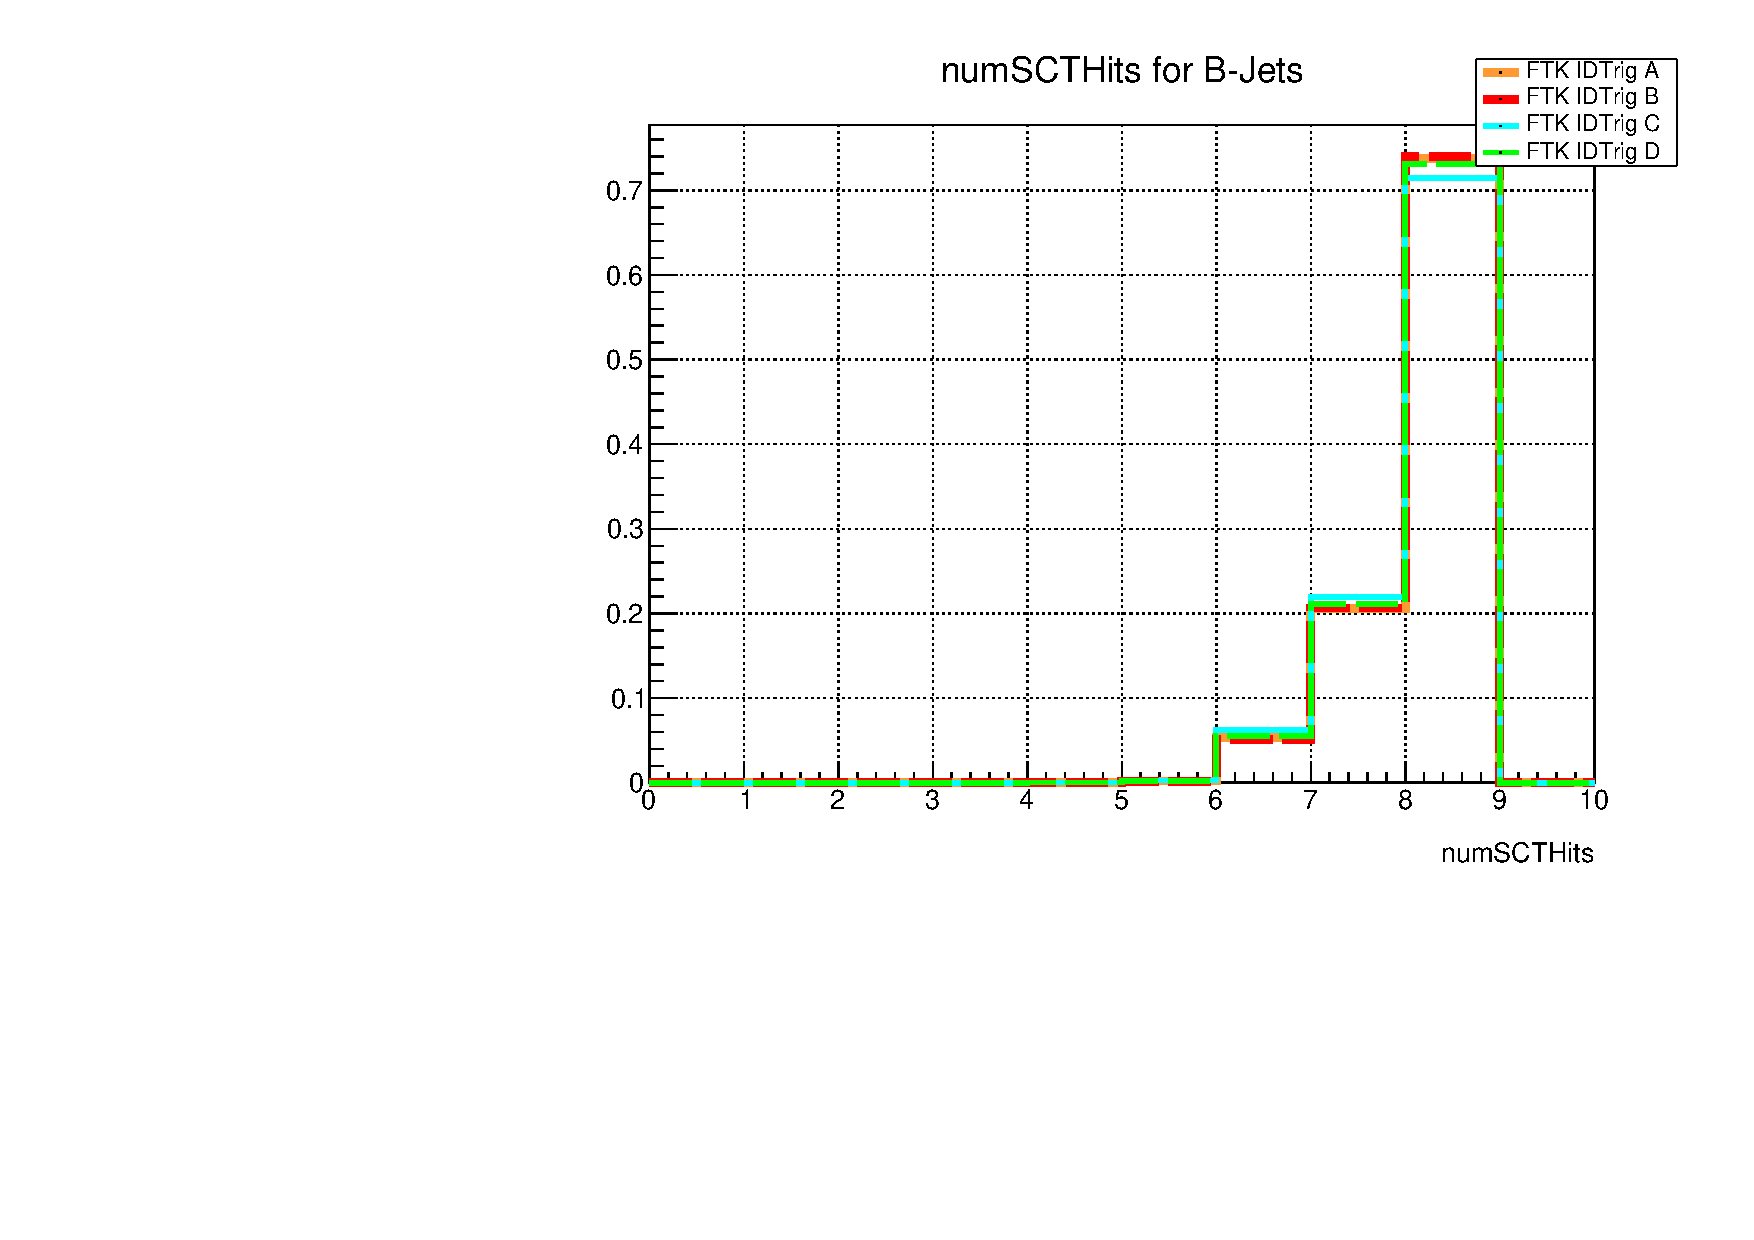
\includegraphics
                [width=\linewidth,height=\textheight,keepaspectratio]
                {correlation_numSCTHits_0}
            \end{figure}
        \end{column}
        \begin{column}{0.33\textwidth}
            \begin{figure}
                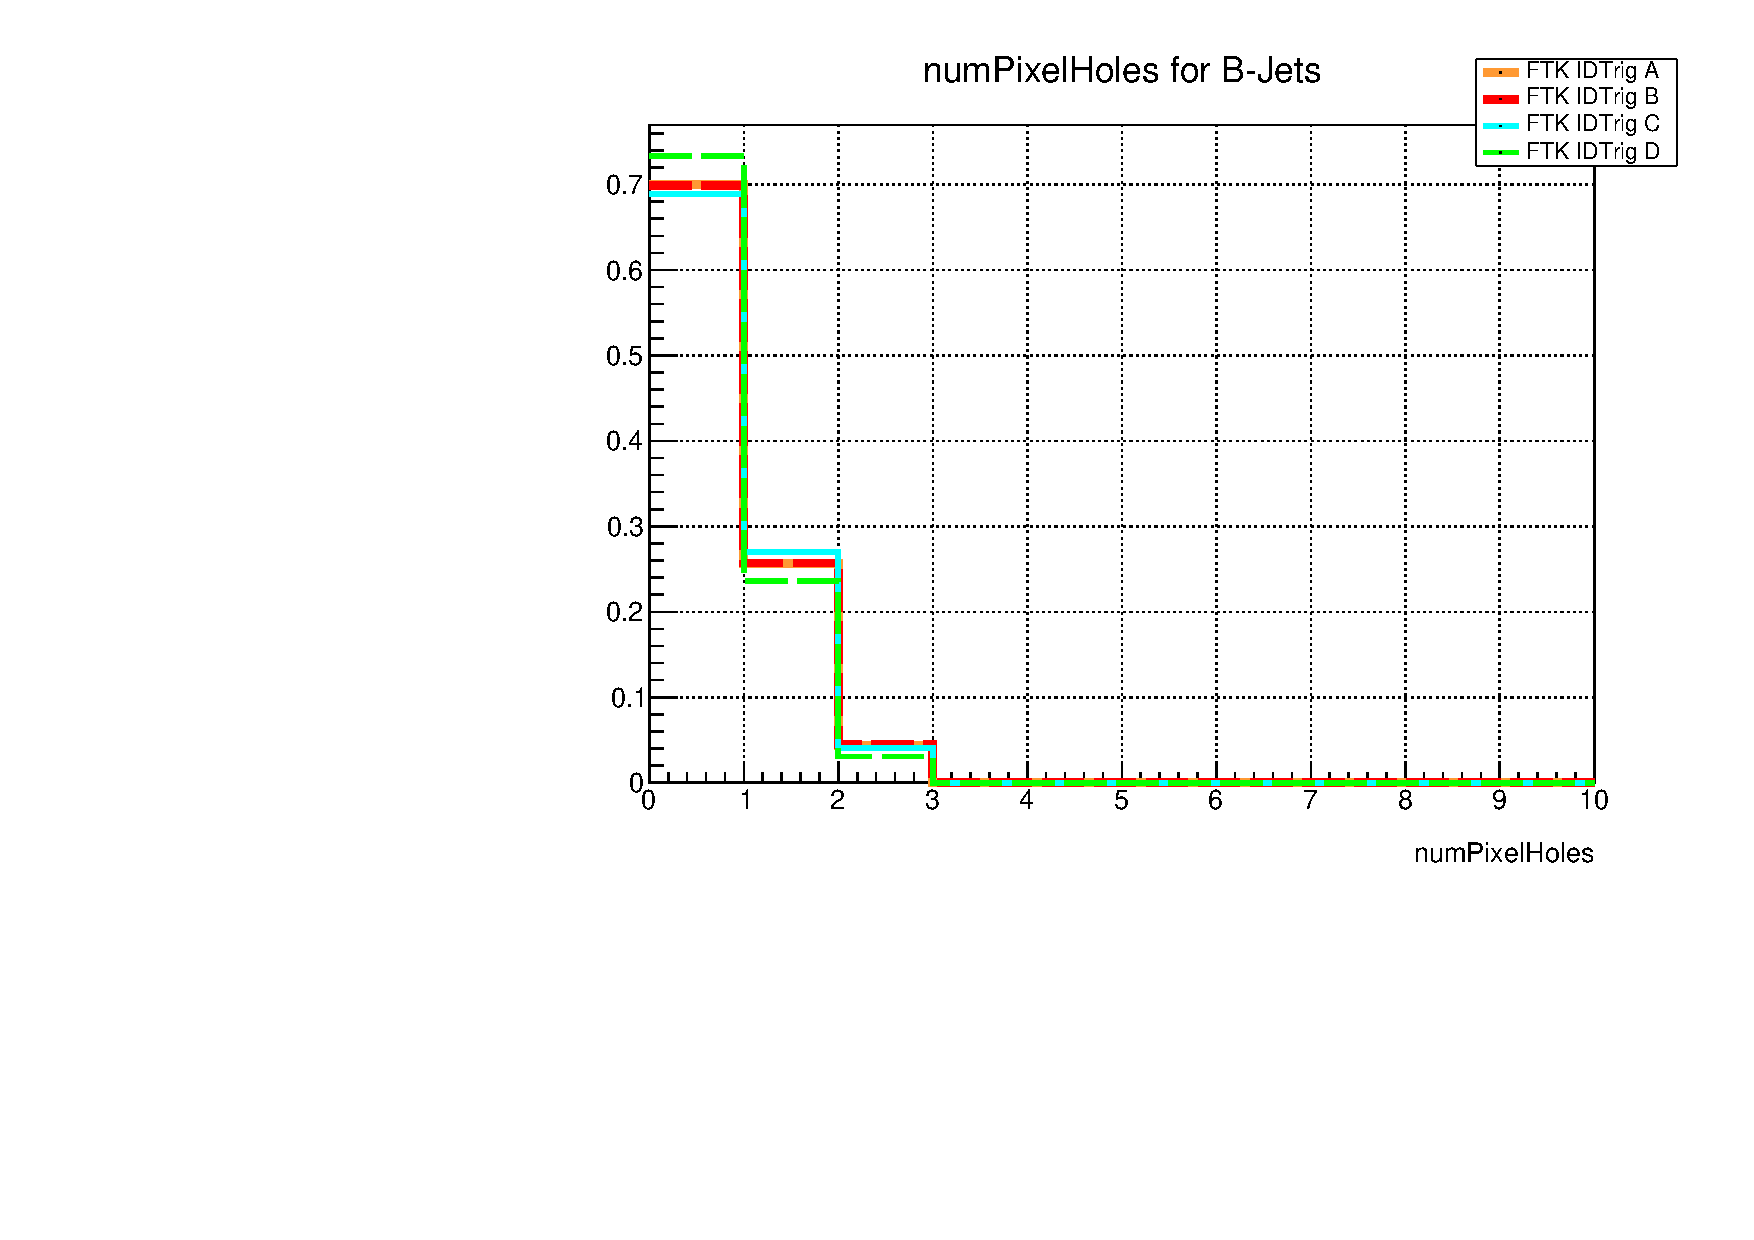
\includegraphics
                [width=\linewidth,height=\textheight,keepaspectratio]
                {correlation_numPixelHoles_0}
            \end{figure}
            \begin{figure}
                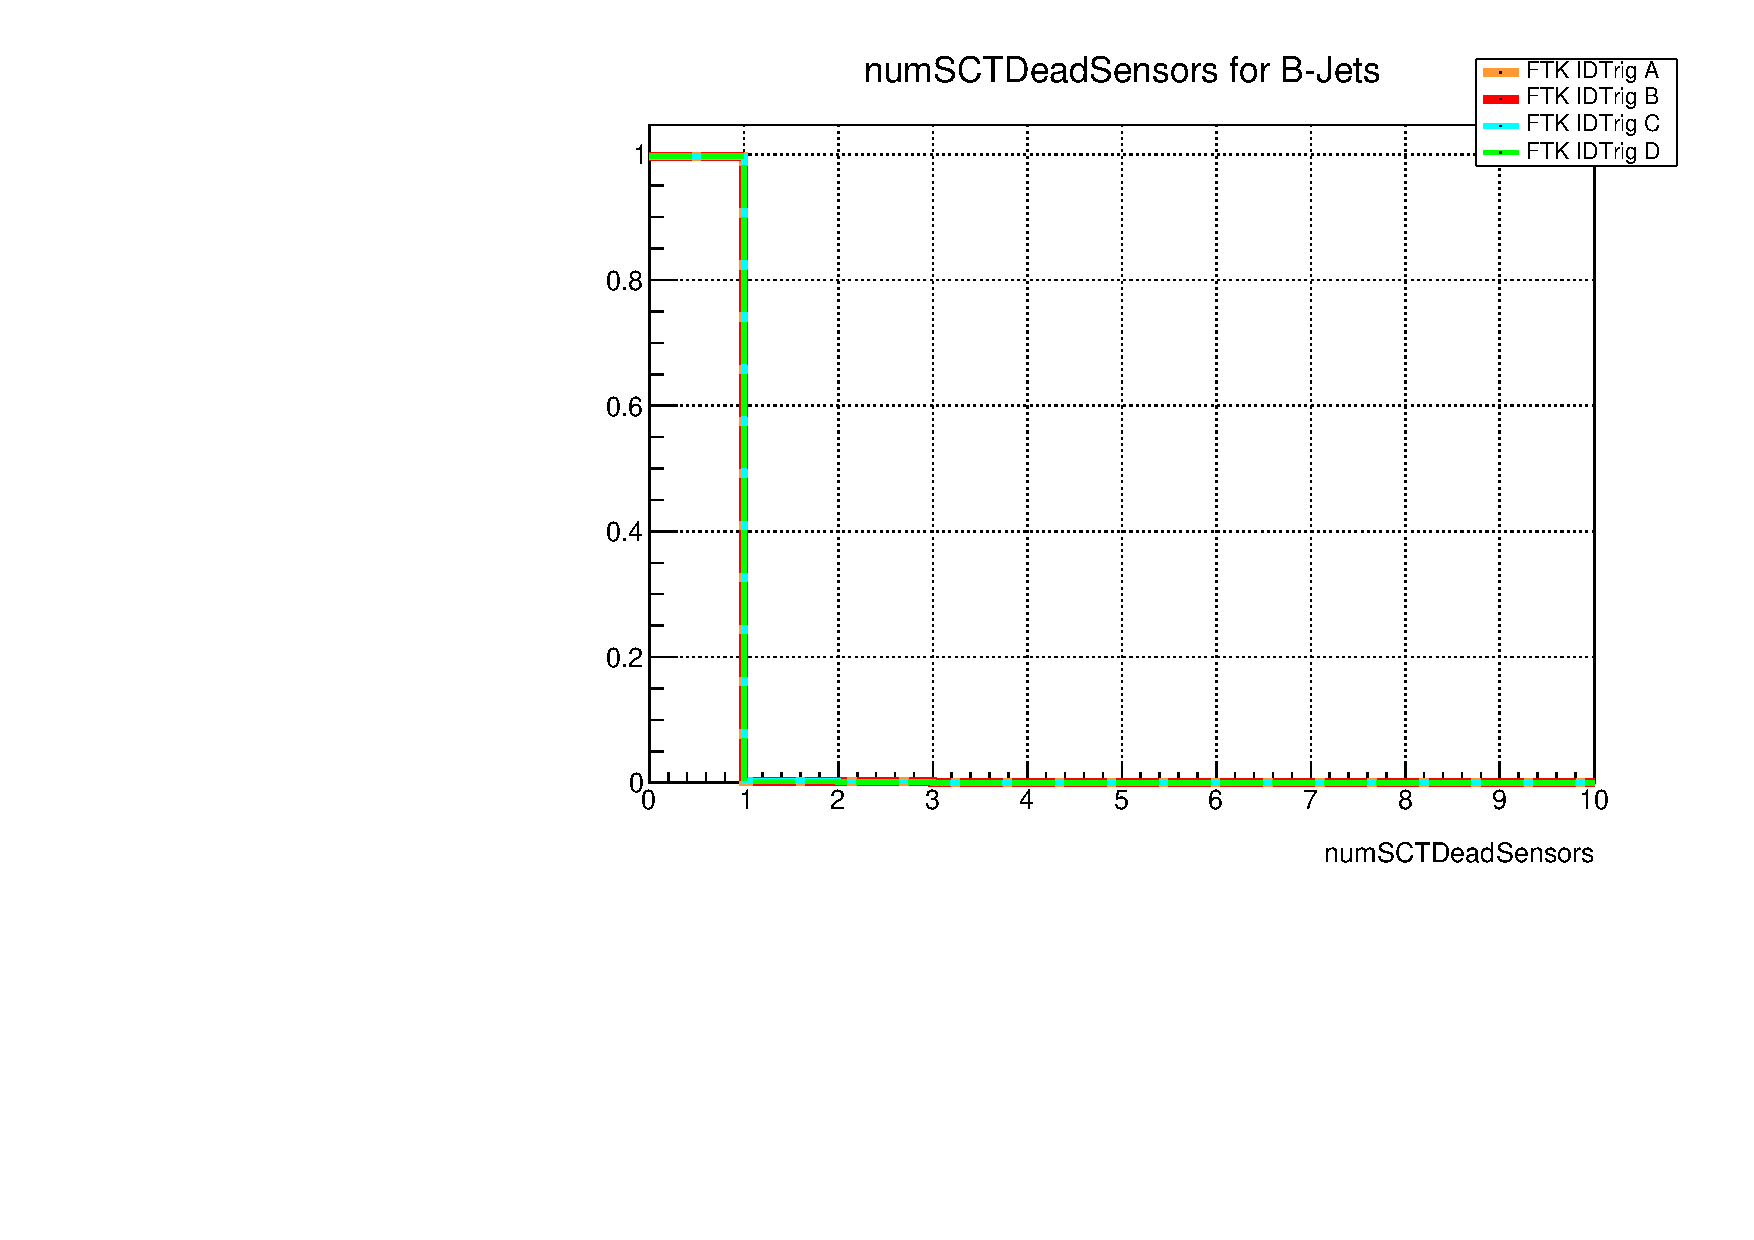
\includegraphics
                [width=\linewidth,height=\textheight,keepaspectratio]
                {correlation_numSCTDeadSensors_0}
            \end{figure}
        \end{column}
    \end{columns}
}

\frame{
    \frametitle{Conclusions}
    \begin{itemize} {\normalsize 
        \item FTK tracks, even with retuning,
            lead to less light-jet rejection in flavour tagging
            compared to the HLT-only counterpart
        \item We want to understand the exact reasons for the observed gap in performance
        \item Comparing track parameters jet-by-jet,
            primary cause appears to be FTK-IDTrig's lower tolerance to small values of d0
        \item This may be related to the apparent ``shift" in d0-error. More studies needed
        \item Track quality values seem to be irrelevant to B-Tagging performance
        \item Additional studies are ongoing. Comments and ideas are welcome
    } \end{itemize}
}

\announcesection{Backup} 
\frame{
    \frametitle{ $T \bar{T}$ Sample and Track Chains Used in this Presentation } 
    Sample T production of four million events:
    { \small mc16\_13TeV.410470.PhPy8EG\_A14\_ttbar\_hdamp258p75\_nonallhad.
        digit.AOD.e6337\_e5984\_s3126\_r11392\_d1512\_r11391 }

    { \tiny (Based on JIRA Ticket: https://its.cern.ch/jira/browse/ATLMCPROD-7318) }

    \vfill

    \begin{table}
    \resizebox{\textwidth}{!}{%
    \begin{tabular}{| l | l | l | l |}
        \hline
        Trigger Title & Input Chain & Track Key & Prm Vtx Key \\
        \hline \hline
        HLT & HLT\_j35\_boffperf\_split & InDetTrigTrackingxAODCnv\_Bjet\_IDTrig & xPrimVx\\
        FTK IDTrig & HLT\_j35\_boffperf\_split\_FTK\_L1J15 & InDetTrigTrackingxAODCnv\_Bjet\_FTK\_IDTrig & PrimVertexFTK\\
        FTKRefit IDTrig & HLT\_j35\_boffperf\_split\_FTKRefit\_L1J15 & InDetTrigTrackingxAODCnv\_Bjet\_FTKRefit\_IDTrig & PrimVertexFTK\\
        %FTK Refit & HLT\_j35\_boffperf\_split\_FTKRefit\_L1J15\_FTK & InDetTrigTrackingxAODCnv\_Bjet\_FTKRefit & PrimVertexFTK\\
        %FTK-HLT & HLT\_j35\_boffperf\_split\_FTKVtx\_L1J15\_FTK & InDetTrigTrackingxAODCnv\_Bjet\_IDTrig & PrimVertexFTK\\
        \hline
    \end{tabular}}
    \end{table}
}

\frame{
    \begin{figure}
    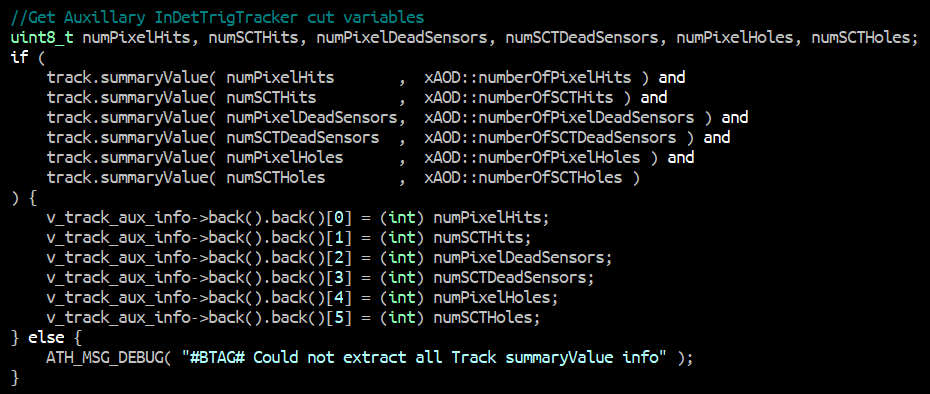
\includegraphics[width=\linewidth,height=\textheight,keepaspectratio]{quality_cut_retrieval}
    \caption{
        \url{https://gitlab.cern.ch/atlas-trigger/b-jet/TrigBtagAnalysis/blob/master/src/BTriggerTuning.cxx\#L1160}
    }
    \end{figure}
}


\displaytwo{Selecting the Appropriate LLR Cut}{}{rejection_level}{rejection_level_zoom}

\displaythree{ d0 Correlation, HLT Distributions }
    { \begin{itemize}
        \item $p_t > 55$ GeV and $|\eta| < 2.5$
        \item Excess Class B at low d0 error may reinforce hypothesis that error shift is responsible,
            but this is still unclear
    \end{itemize} }
    {track_study/plot_hlt_correlation_d0_0}
    {track_study/plot_hlt_correlation_d0_err_0}
    {track_study/plot_hlt_correlation_d0_sig_0}

\displaythree{ $\theta$ Correlation, HLT Distributions }
    { \begin{itemize}
        \item $p_t > 55$ GeV and $|\eta| < 2.5$
    \end{itemize} }
    {track_study/plot_hlt_correlation_theta_0}
    {track_study/plot_hlt_correlation_theta_err_0}
    {track_study/plot_hlt_correlation_theta_sig_0}

\end{document}

